\documentclass[titlepage, 12pt]{article}

\title{

\includegraphics[width=.3\textwidth]{cvut-logo.jpg}\par
\vspace{10mm}
\indent
\textbf{CZECH TECHNICAL UNIVERSITY IN PRAGUE}

FACULTY OF TRANSPORT SCIENCES

\vfill

{\Large JAN MACEK}
\vspace{10mm}

AGENT-BASED MODELING OF ITS SYSTEMS IN VEHICLE SIMULATOR 
\vspace{15mm}

{\Large DIPLOMA THESIS}
\vfill

}
\date{\Large 2022}

\usepackage[utf8]{inputenc}
\usepackage{listings}
\usepackage{fancyhdr}
\usepackage{graphicx}
\usepackage{parskip}
\usepackage{svg}
\usepackage[a4paper, top=25mm, bottom=25mm, left=30mm, right=20mm, twoside]{geometry}
\usepackage{tabularx}
\usepackage{caption}
\usepackage{hyperref}
\usepackage{xcolor}
\usepackage{amsmath}
\usepackage[sorting=none]{biblatex} 
\usepackage{color}
\usepackage{pdfpages}
\usepackage{enumitem}
\usepackage{amssymb}
\usepackage{booktabs}
\usepackage{microtype}
\usepackage{subfiles}
\usepackage{multirow}
\usepackage{pdfpages}
\usepackage{enumitem}

\definecolor{dkgreen}{rgb}{0,0.6,0}
\definecolor{gray}{rgb}{0.5,0.5,0.5}
\definecolor{mauve}{rgb}{0.58,0,0.82}
\definecolor{inline}{rgb}{0.25,0.25,0.80}


\addbibresource{references.bib}

\hypersetup{
    colorlinks,
    linkcolor={red!50!black},
    citecolor={blue!50!black},
    urlcolor={blue!70!black}
}

\pagestyle{fancy}

\graphicspath{{./img}}

\fancyhead[L]{Jan Macek}
\setlength{\headheight}{15pt}

\newlength{\varSepscale}
\setlength{\varSepscale}{16pt}
\newcommand{\itemspacing}[1]{\setlength\itemsep{\dimexpr #1\varSepscale-\varSepscale}}
\newcommand{\term}[1]{\hspace*{2em}\textit{#1}\, -\,}
\newcommand{\rot}[1]{\rotatebox[origin=c]{90}{#1}}
\newcommand{\talign}[3]{\makebox[#2em]{#1\hfill}#3}

%DOCUMENT
\begin{document}
\setlength{\baselineskip}{1.5em}
\maketitle

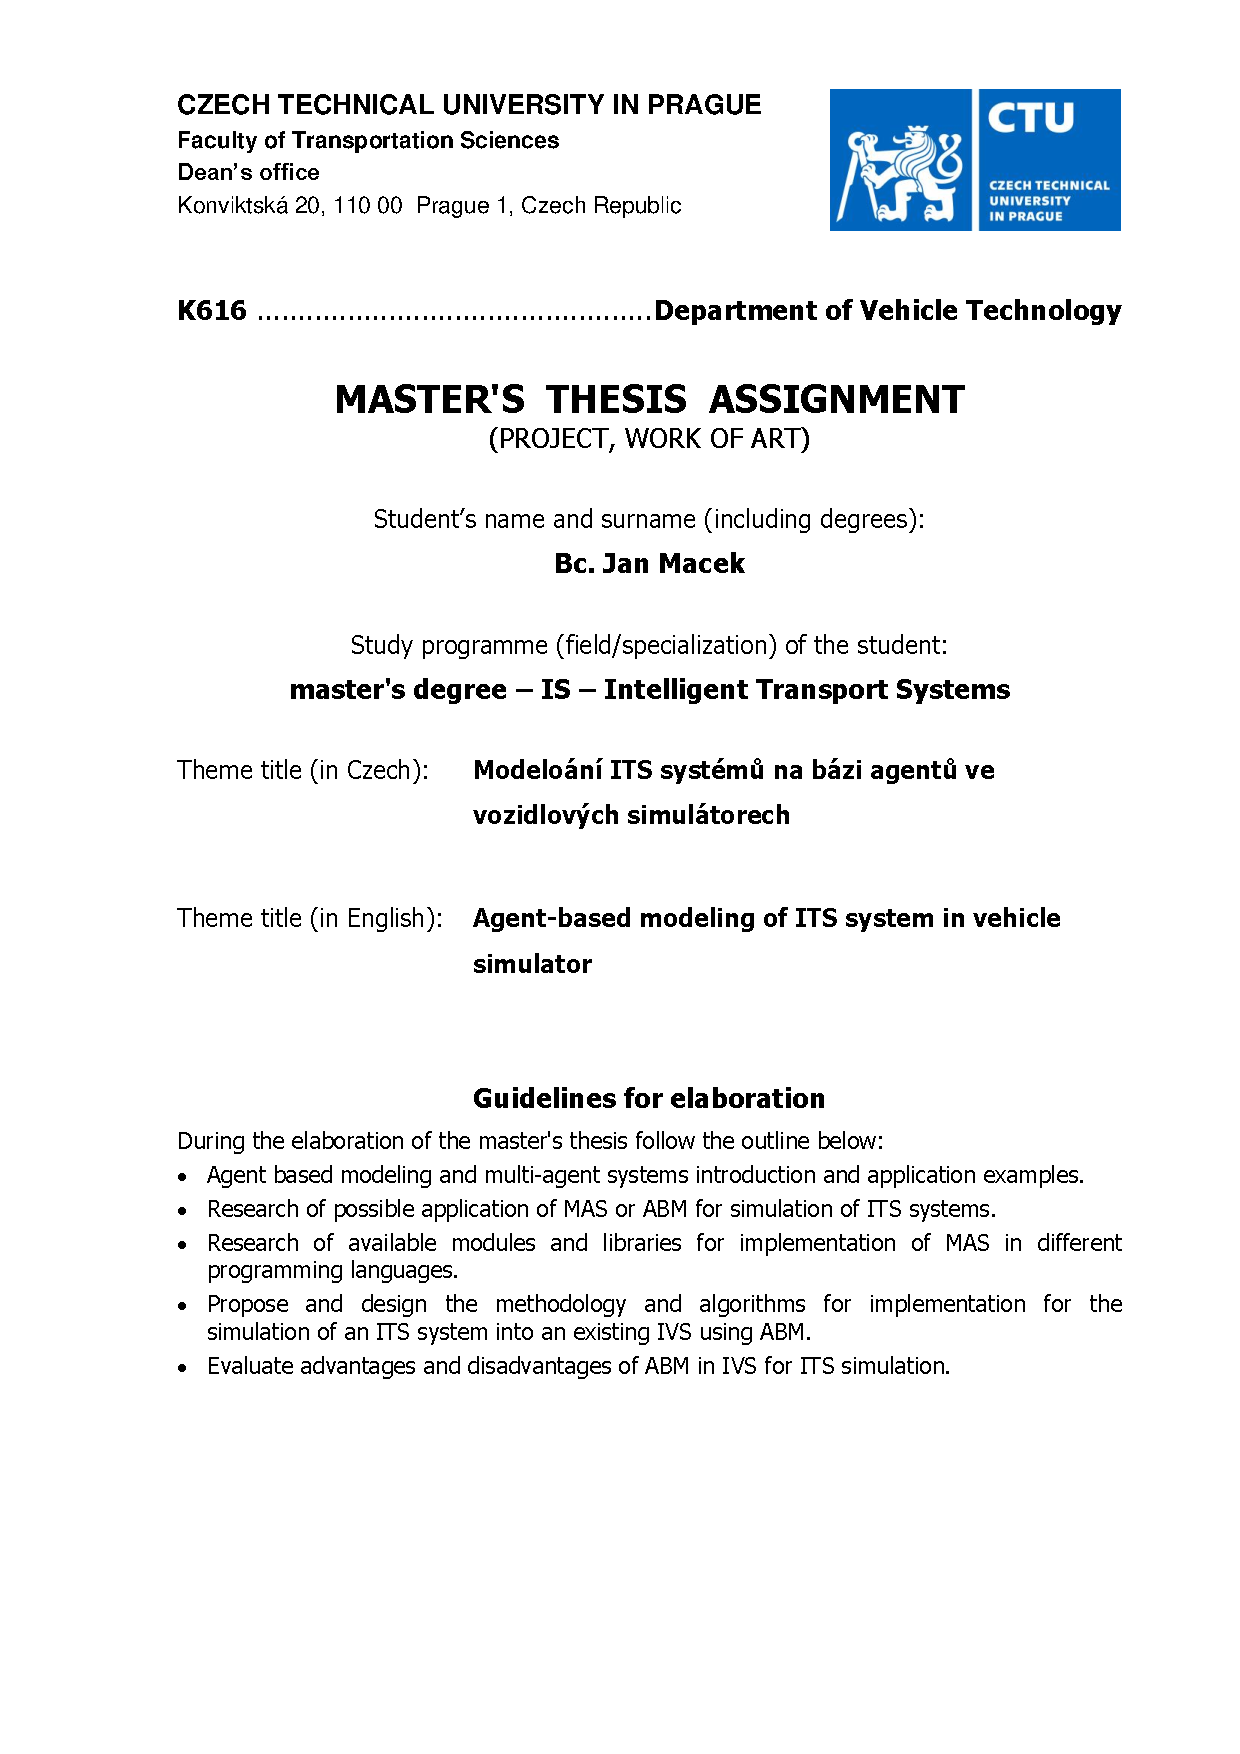
\includepdf[pages=-]{zadani-dp-jan-macek.pdf}

\begin{abstract}
    TODO
\end{abstract}

\tableofcontents
\newpage

\section{Introduction}

In a world where vehicle transport plays an inseparable role in the society, with an ever increasing
demand, it is important to analyze and study driver behaviour and inherently interactions and
relationships between drivers and their surroundings. This is supported by the fact that, even though
substantial advancements in autonomous driving are being made, for the near-future, humans will still
have to control vehicles themselves and therefore be exposed to a substantial risk of danger. 
Data shows that about 95 \% of traffic accidents are a result of human error \cite{Parliament2021}. 
Each traffic accident has got a tremendous effect on socio-economic growth. A study be the European
Union states that accident-related expenses (including cost of fatality) cost 1,8 \% of EU GDP \cite{Wijnen2017}.  
A rather non-cynical point of view is that each life lost is a failure in society itself and an effort
should be made to diminish fatal accidents.

A method that has proven to be effective at studying driver behaviour and
traffic safety is by using interactive vehicle simulators (IVS), which allow to
undertake experiments in a safe, controlled and reproducible way.  Because
driving simulator is basically a digital twin of a real vehicle, it is naturally
reasonable to make the interaction between the driver and IVS as close to
reality as possible, which inherently improves data quality of the simulation
and potentially also the range of IVS application. An IVS has got a broad
spectrum of employment. It is not only used as a tool to research driver
behaviour, but also used in development and testing of advanced
driver-assistance systems, extending the simulator to a hardware-in-the-loop or
a vehicle-in-the-loop system, which enables to test real hardware and simulate
full road testing.

Simulating the traffic environment is a complex problem, mainly because of
its highly dynamic characteristics. All vehicles  need to interact with
each other and act upon other drivers' actions. Because agent-based simulations
have proven to model complex behaviour well, this modelling technique seems like
a suitable solution for achieving a realistic traffic environment for IVS.

The goal of this thesis is to investigate multi-agent systems (MAS), their 
principles and evaluate usages of these systems related to ITS research, where 
their shared characteristics of distributed interoperability could prove to make 
agent-based modelling a strong tool for simulating ITS solutions. The output of 
the experimental/practical part of the thesis should be A MAS-based simulation framework 
for facilitating and streamlining the process of ITS solutions simulation.

In the first two chapters, a review of the state-of-art research about Intelligent 
Transport Systems and Multi-agent Systems is presented, with an emphasis on the 
respective field's system model point of view. In the third chapter, requirements 
for the proposed framework are specified, based on the preceding research. In the 
fourth section, a self-proposed framework architecture is proposed, in line with 
MAS paradigms and adapted for ITS solutions simulation. In the fifth section, the
implementation requirements are specified, mainly discussing the simulator software integration
and additional development platforms and libraries that could potentially facilitate the
framework design process. In the sixth section, a technical implementation of the 
framework is presented, showing the implementation details while also serving as the 
software's documentation. In section number seven, a validation of the proposed 
system is conducted by implementing a distributed cooperative ITS system into an 
IVS, using the proposed framework and assessing its performance and overall results.

\subfile{1its}

\subfile{2mas}

\subfile{3requirements}

\subfile{4system}

\subfile{5toolset}

\subfile{6implementation}

\subfile{7validation}

\clearpage

\printbibliography
\end{document}
